% Base shape
\tikzstyle{layer} = [rectangle, draw, minimum height=2em, text centered, rounded corners]
\tikzstyle{arrow} = [thin,->,>=stealth]

% Specific shapes
\tikzstyle{io}    = [layer, fill=gray!20]
\tikzstyle{conv}  = [layer, fill=green!20]
\tikzstyle{dense} = [layer, fill=red!20]
\tikzstyle{lstm}  = [layer, fill=blue!20]

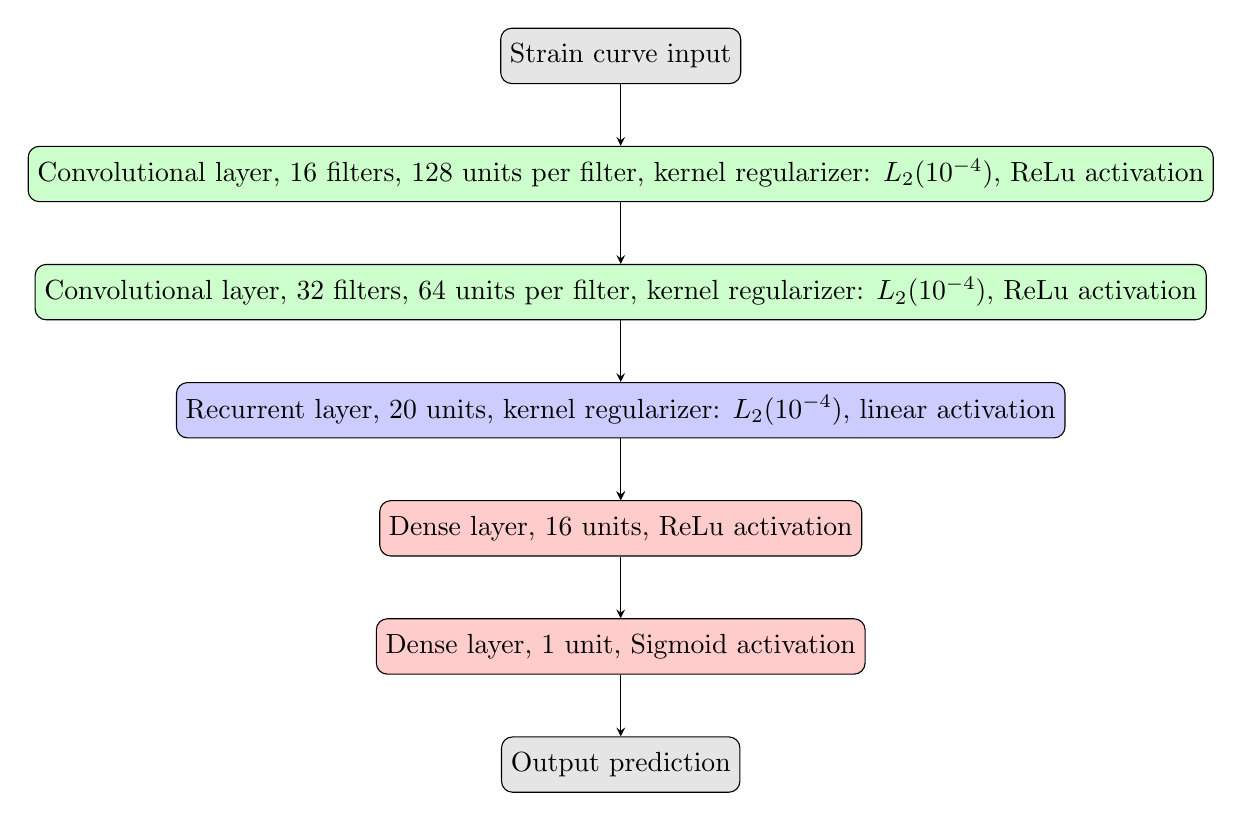
\begin{tikzpicture}
\node (input)  [io] {Strain curve input};
\node (conv1)  [conv,  node distance=1.5cm, below of=input]  {Convolutional layer, 16 filters, 128 units per filter, kernel regularizer: $L_2 (10^{-4})$, ReLu activation};
\node (conv2)  [conv,  node distance=1.5cm, below of=conv1]  {Convolutional layer, 32 filters, 64 units per filter, kernel regularizer: $L_2 (10^{-4})$, ReLu activation};
\node (lstm)   [lstm,  node distance=1.5cm, below of=conv2]  {Recurrent layer, 20 units, kernel regularizer: $L_2 (10^{-4})$, linear activation};
\node (dense1) [dense, node distance=1.5cm, below of=lstm]   {Dense layer, 16 units, ReLu activation};
\node (dense2) [dense, node distance=1.5cm, below of=dense1] {Dense layer, 1 unit, Sigmoid activation};
\node (output) [io,    node distance=1.5cm, below of=dense2] {Output prediction};

\draw [arrow] (input) --node {} (conv1);
\draw [arrow] (conv1) --node {} (conv2);
\draw [arrow] (conv2) --node {} (lstm);
\draw [arrow] (lstm) --node {} (dense1);
\draw [arrow] (lstm) --node {} (dense1);
\draw [arrow] (dense1) --node {} (dense2);
\draw [arrow] (dense2) --node {} (output);
\end{tikzpicture}
